\documentclass[msc,lith,english]{liuthesis}
  %% Settings go in settings.tex
  %%% settings.tex --- 
%% 
%% Filename: settings.tex
%% Description: 
%% Author: Ola Leifler
%% Maintainer: 
%% Created: Tue Oct 19 21:11:31 2010 (CEST)
%% Version: $Id$
%% Version: 
%% Last-Updated: Tue Apr 25 08:49:48 2017 (+0200)
%%           By: Ola Leifler
%%     Update #: 43
%% URL: 
%% Keywords: 
%% Compatibility: 
%% 
%%%%%%%%%%%%%%%%%%%%%%%%%%%%%%%%%%%%%%%%%%%%%%%%%%%%%%%%%%%%%%%%%%%%%%
%% 
%%% Commentary: 
%% 
%% 
%% 
%%%%%%%%%%%%%%%%%%%%%%%%%%%%%%%%%%%%%%%%%%%%%%%%%%%%%%%%%%%%%%%%%%%%%%
%% 
%%% Change log:
%% 
%% 
%% RCS $Log$
%%%%%%%%%%%%%%%%%%%%%%%%%%%%%%%%%%%%%%%%%%%%%%%%%%%%%%%%%%%%%%%%%%%%%%
%% 
%%% Code:
\usepackage[backend=biber, hyperref, sorting=none]{biblatex}
\usepackage{todonotes}
\usepackage{bm}
\usepackage{subcaption}
%% To set the font of your thesis, use the \setmainfont{} command,
%% surrounded with \ifxetex if you want to switch between xelatex and pdflatex
\ifxetex 
%\setmainfont [Scale=1]{Georgia}
\fi
%%%%%%%%%%%%
%% The VZ43 chapter style, from Memoir contributed chapter styles: ftp://ftp.tex.ac.uk/ctan%3A/info/MemoirChapStyles/MemoirChapStyles.pdf
%%%%%%%%%%%
\usepackage{calc,color}
\DeclareMathOperator*{\argmin}{arg\,min}
\DeclareMathOperator*{\argmax}{arg\,max}
\newif\ifNoChapNumber
\newcommand\Vlines{%
\def\VL{\rule[-2cm]{1pt}{5cm}\hspace{1mm}\relax}
\VL\VL\VL\VL\VL\VL\VL}
\makeatletter
\setlength\midchapskip{0pt}
\makechapterstyle{VZ43}{
\renewcommand\chapternamenum{}
\renewcommand\printchaptername{}
\renewcommand\printchapternum{}
\renewcommand\chapnumfont{\Huge\bfseries\centering}
\renewcommand\chaptitlefont{\Huge\bfseries\raggedright}
\renewcommand\printchaptertitle[1]{%
\Vlines\hspace*{-2em}%
\begin{tabular}{@{}p{1cm} p{\textwidth-3cm}}%
\ifNoChapNumber\relax\else%
\colorbox{black}{\color{white}%
\makebox[.8cm]{\chapnumfont\strut \thechapter}}
\fi
& \chaptitlefont ##1
\end{tabular}
\NoChapNumberfalse
}
\renewcommand\printchapternonum{\NoChapNumbertrue}
}
\makeatother

\newtheorem{definition}{Definition}

%% To set bibliography options, refer to the biblatex manual and use
%% the ExecuteBibliographyOptions command below to set your options
\DeclareFieldFormat{urldate}{%
(Accessed: \thefield{urlday}\addspace%
\mkbibmonth{\thefield{urlmonth}}\addspace%
\thefield{urlyear}\isdot)}
\ExecuteBibliographyOptions{maxnames=99}
%% Change this to your appropriate BibTeX reference file (.bib)
\addbibresource{references.bib}
%%%%%%%%%%%%%%%%%%%%%%%%%%%%%%%%%%%%%%%%%%%%%%%%%%%%%%%%%%%%%%%%%%%%%%
%%% settings.tex ends here
%%% Local Variables: 
%%% mode: latex
%%% TeX-master: "demothesis"
%%% End: 
  \usepackage{rotating}
  \usepackage{color}
  % \usepackage{changebar}
  \department{Institutionen för datavetenskap}
  \departmentenglish{Department of Computer and Information Science}
  \departmentshort{IDA}
  % If this is a thesis at the cognitive science study programme, use
  % the "area" command to generate a proper (?) ISRN
  % \area{KOGVET-A}
  % Include an external supervisor on the cover page
  \externalsupervisor{Simon Johansson}
  \supervisor{Mattias Tiger}
  \examiner{Fredrik Heintz}
  \titleenglish{BEAUTIFUL TITLE, ENGLISH}
  \titleswedish{VÄLDIGT FIN TITEL}
  \thesissubject{Computer Science}
  \publicationyear{2018}
  \currentyearthesisnumber{XXX}
  \dateofpublication{\today}
  \author{Linus Kortesalmi}
  % Two authors
  % \author{\parbox{\textwidth}{Ola Leifler\\
  %   Alexander Sanner}}
  \begin{document}

  \chapterstyle{VZ43}
  \chapter{Introduction}
\label{cha:introduction}

% Smartphones have given hackers new appealing attack vectors to exploit \cite{Nokia2016}.
% One of these attack vectors is the publishing of malicious applications that act like benevolent ones.
% These applications are commonly referred to as Potentially Harmful Applications (PHAs) \cite{PHA}.
% For example, PHAs could be disguised Trojans stealing the consumer's contact information, opening backdoors on the infected device or even sending SMS messages \cite{current-android-malware}.

% Google releases annual Android security reports covering different security aspects tackled throughout the year.
% In Google's Android security report from 2015 \cite{android-security-2015}, they stated that "less than 0.5\% of devices had a PHA installed" and that this number was 0.15\% for devices that only installed applications from Google's own application store, Google Play\footnote{https://play.google.com/store?hl=en}.
% In Google's review of 2016 \cite{android-security-2016} the average increased to 0.71\% of devices, while the percentage was reduced to 0.05\% for the devices installing exclusively from Google Play.
% The increase of PHAs in devices installing applications from other sources than Google Play is interesting, as it might be indicative of a change in user behaviour, or the result of an increase of PHAs in other application stores.
% It is, however, clear that the threat from PHAs still exists in 2017.

Maintenance of devices/vehicles/systems/machines (hereinafter referred to as “units”) is generally done by planned scheduling. 
Typically this is done when some parameter of the system reaches a threshold value. 
For example, car maintenance can be scheduled after 30,000 kilometres, after a year or perhaps after a certain number of operating hours.
One problem with planned scheduling is the reliance on experience and statistics from many units.
For a single unit, the planned scheduling will either be executed too early (could have waited longer before service) or too late (problems encountered before threshold reached).

Internet of Things (IoT) permits the streaming of continuous data from multiple units.
The data is typically the state of the unit in the shape of many different variable values.
A rule framework can be built incorporating the continuous data.
The framework can then give an informed service alert based on the actual state and need of a unit.

Machine Learning (ML) models can be used to, for example, capture dependencies in large-scale data sets (ref needed), anomaly detection (ref), clustering (ref), image recognition (ref), and decision making (ref). 
Anomaly detection could be used together with continuous real-time data from a system to find unusual changes or behaviour, which could be the basis for a service alert and/or the gathering of new knowledge about a system.
ML-algorithms can also be used to perform Predictive Maintenance (PdM).

\section{Background}

\subsection{Maintenance Techniques}
There are different techniques to carry out maintenance work, each with various drawbacks and benefits.
Corrective Maintenance (CM) is the technique to identify, isolate, and solve faults.
The aim of CM is to restore the faulty equipment to working conditions.
CM can only be done after a fault has been detected and is a reactive approach to maintenance.
The fault detection can be carried out without the need of expensive, or extensive, equipment to monitor the health of a system.
On the other hand, such equipment can help during the fault identification and isolation steps. \todo{source}
The faults typically require costly repairs or equipment replacement, as small failures might not be detected until a major fault occurs.

Another technique is Preventive Maintenance (PM).
PM focuses on proactive maintenance of equipment by carefully monitoring and servicing equipment by expert personnel.
The goal is to maintain satisfactory operating conditions of the system by solving minor faults before they cause major ones.
PM requires good knowledge about the system and regular, systematic inspections to be carried out.
% Dyrt att underhålla på detta vis, men leder kanske ofta till att system inte går ner lika mycket som i CM (då system alltid går ner innan problem fixas)
% Valet mellan dessa beror på industrin du arbetar inom.

The technique which will be explored in this thesis is Predictive Maintenance (PdM).
The aim of PdM is to optimise scheduled maintenance work and minimise, or even prevent, unexpected equipment failures.
Equipment is directly monitored and measured to understand the actual maintenance need.
Maintenance can then be scheduled for a specific equipment, based on the actual need.

\subsection{Internet of Things}
Internet of Things (IoT)

\section{Problem Description}
\label{sec:problem-description}
% The problem of malware existed long before the invention of smartphones.
% The antivirus (AV) industry has been combatting this issue for decades.
% Modern AV software use different approaches, like signature-based detection or heuristics, to detect malware in computers.
% One of the problems with signature-based detection is the tools available for hackers to alter the code of a malicious programme, which would change the signature of the programme.
% This could, for example, be done by using metamorphic virology \cite{metamorphic-virology}.
% The heuristic approach tries to capture the essence of malicious programmes and group similar malware together.
% The grouping is done by manually engineering generic signatures for the malware.
% This manual labour required to engineer generic signatures, together with the rapid evolution of malware, make heuristics an infeasible long-term solution.
% Today, effort is put into using machine learning algorithms to detect malware.
% Some of the algorithms used are: Naive Bayes (NB) classifier \cite{Shang2017}, Support Vector Machines (SVMs), Random Forest (RF) classifiers and Convolutional Neural Networks (CNNs) \cite{McLaughlin2017}. 

\section{Aim}
\label{sec:aim}
The expected results is a study on how ML-algorithms can be used for Predictive Maintenance (PdM).
The study shall compare at least two different ML-algorithms.
The goal is to implement the ML-algorithms and use real-world data from an existing IoT system.
The aim of the study is also to compare how well the improved DcM performs with the current solution used in the IoT system (preliminary, more info needed from company as well as ideas how to compare the solution with the practice in use today).

% This work aims to use the NB, SVMs, RF classifiers and CNNs to detect malicious Android Package Kits (APKs).
% The algorithms are implemented and then evaluated by comparing their accuracy (the fraction of malicious APKs found) with the number of false positives (benign APKs falsely flagged as malicious).
% The specific metrics used are covered in Section \ref{sec:eval-metrics}.
% The classifiers use static APK features for training, validation and testing.

\section{Research Questions}
\label{sec:research-questions}
This work explicitly answers the following questions:
\todo{The RQs below are just an initial draft.}
\begin{enumerate}
  \item Which methods can be used to detect anomalies in a dynamic real-time system?
  \item How can the need for maintenance be detected from real-time processing of (domain-specific) data?
  \item How can predictive maintenance be achieved by processing real-time (domain-specific) data?
  \item How far in advance can maintenance be predicted?
%   \item How does the NB classifier perform compared to SVMs or RF classifiers with respect to accuracy and precision?
%   \item How can static APK features be used to train a CNN?
%   \item How do CNNs perform compared to NB, SVMs and RF classifiers, with respect to accuracy and precision?
%   \item Which features, other than static APK features, could potentially be useful when classifying malicious applications?
\end{enumerate}

\section{Delimitations}
\label{sec:delimitations}
% Only static APK features are used for actual training; the discussion of alternative features is only theoretical.
% The specific implementations used of the NB classifiers, SVMs, RF classifiers and CNNs are not covered in detail.
% However, the parameters chosen for each algorithm are presented and discussed in detail.
% Algorithms are only evaluated based on their accuracy and the number of false positives classified.

  \chapter{Background}
\label{cha:background}

\section{Gaussian Processes}
In \cite{Rasmussen2004} everything we need to know about Gaussian Processes (GP) is written, good huh? \todo{Obviously edit this and fill out the section!}

\section{Combining GPs}
\todo{...}

\section{Exploratory Data Analysis}
Exploratory Data Analysis (EDA) is a broad concept containing various techniques \cite{Anselin1999, Gelman2003, Hoaglin2003, Tukey1977, Velleman1981} for exploring and analysing data.
Early popular techniques include \emph{box plots} and \emph{stem-and-leaf} displays.
A stem-and-leaf plot takes numbers and splits them into two groups.
The first group contains the leading digit(s) and the second group contains the trailing digit(s).
Figure \ref{fig:stem-leaf-plot} is an example of a stem-and-leaf plot with one leading and one trailing digit.
The grouping helps when sorting batches of data and visualising important features, without losing the information of every single data point used \cite{Velleman1981}.

\begin{figure} [h!]
    \centering
    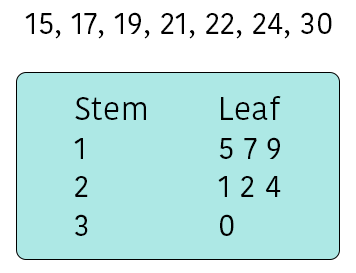
\includegraphics[width=0.33\textwidth]{figures/stem-leaf-plot}
    \caption{Example of a stem-and-leaf plot. The numbers above the plot is the input.
    The first digit of the number is the \emph{stem}, the following digits are the \emph{leafs}.}
    \label{fig:stem-leaf-plot}
\end{figure}

EDA can be seen as applying tools and statistics to analyse data in a meaningful way, e.g., it could be applied to the detection of outliers, smoothing the data, and performing a variance analysis \cite{Anselin1999, Hoaglin2003, Tukey1977, Velleman1981}.
EDA can also reveal subtle practical problems with the chosen model that can easily be missed when performing statistical theory analysis of the model \cite{Gelman2003}.

In \cite{Tukey1977}, Tukey describes how EDA can be used to answer research questions such as "What is the age distribution for the Vietnamese population?" and "Are there differences in
the annual household per capita expenditures between the rural and urban populations in Vietnam?".
Tukey uses plots to compare different groups and estimators to quantify the difference.
For example, the sample mean estimator, or the \emph{winsorised} mean can be used \cite{Tukey1977}.
The winsorised mean handles the case where tails of a distribution dominates the value space.  
This would cause the sample mean estimator to poorly reflect on the "typical" data point, as it is skewed by the small tail population \cite{Tukey1977}.

In \cite{Velleman1981}, Velleman et al. present different EDA techniques and highlights four key areas of EDA: displays (plots), residuals, re-expressions and resistance.
Residuals is what remains after data analysis is performed.
Residuals could, for example, be what remains after fitting data to a model (the error of the fit) \cite{Velleman1981}.
Re-expression is the notion of applying mathematical functions to the data.
Re-expressing the data can help with the data analysis \cite{Hoaglin2003, Velleman1981}.
Examples of mathematical functions that can be applied are: logarithm, square root, reciprocal square function or generally raising the data to some power $p$.
Resistance is the concept that outliers should not disproportionately affect the data analysis \cite{Hoaglin2003, Velleman1981}.
For example, the winsorised mean estimator would be less sensitive to localised misbehaviour than the sample mean estimator \cite{Tukey1977}.

Smoothing data is important for many different applications \cite{Bradley1997, Pang2002, Quinlan1992, Velleman1981}.
This can, for example, be done by applying \emph{running median smoothers}.
The running median smoothers go through all the data points in sequence and calculate only the median for the $n$ closest values near each point \cite{Velleman1981}.
Another approach is the \emph{running weighted average} \cite{Velleman1981}.
Instead of taking the median of the $n$ values, the average is calculated.
The average can also be weighted with different functions, like hanning smoothing \cite{Velleman1981}.
The hanning smoothing for three data points is shown in Eq. \ref{eq:hanning}.
It is worth noting that a single outlier will heavily affect the hanning smoothing and that in practice it is common to first apply a running median smoothing to remove outliers \cite{Velleman1981}.

\begin{equation}
    \hat y_t = \frac{1}{4} y_{t-1} + \frac{1}{2} y_t + \frac{1}{4} y_{t + 1} 
    \label{eq:hanning}
\end{equation}
  \chapter{Data}
\label{cha:data}

This chapter describes the spatio-temporal dataset used in the thesis project.
The dataset provider is briefly mentioned alongside the data gathering process, followed by the structure of the data.
The different event types in the dataset are described and how they are used in the thesis project.
A pre-study of the dataset is detailed after the basic characteristics of the dataset have been described.
The dataset pre-study analysed the data in-depth and identified problems which occur because of the basic characteristics and their limitations.
The problems are illustrated by real-world examples.
The pre-processing section covers methods employed to transform the data into usable features.
The pre-processing section also mentions solutions to some of the problems identified in the dataset pre-study.

\section{Background}
The dataset is provided by Östgötatrafiken AB and contains 282 GB of data.
Östgötatrafiken AB is owned by Östergötland County and is responsible for the public transportation in the county.
During this thesis project, only the bus data available in the given data set is analysed.
The dataset is a collection of documents, where one document represents a full day of data.
The dataset contains 62 days.
A typical day has a document size of around 5 GB, see Figure \ref{fig:log-sizes}.

\subsection{Traffic Lab}
Traffic Lab API\footnote{https://www.trafiklab.se/} contains complementary information to the data in the provided dataset by Östgötatrafiken AB.
For example, one can retrieve coordinates for all bus stops and the arrival times for buses at each bus stop.
However, the arrival times are not updated in real-time for the buses of Östgötatrafiken AB.

\subsection{Data Gathering}
The process of gathering the data used in this thesis project can be generally described by the following simplified procedure:
\begin{enumerate}
    \item Each Östgötatrafiken AB bus is running a system collecting data from sensors installed inside the bus.
    \item The system collects the sensor data and transmits it to a central server or database.
    \item A log containing all events for a full day is created and stored as a document in a collection.
    \item The central server processes and analyses the data.
    The results from the data analysis is stored in the log.
\end{enumerate}

\begin{figure}
    \centering
    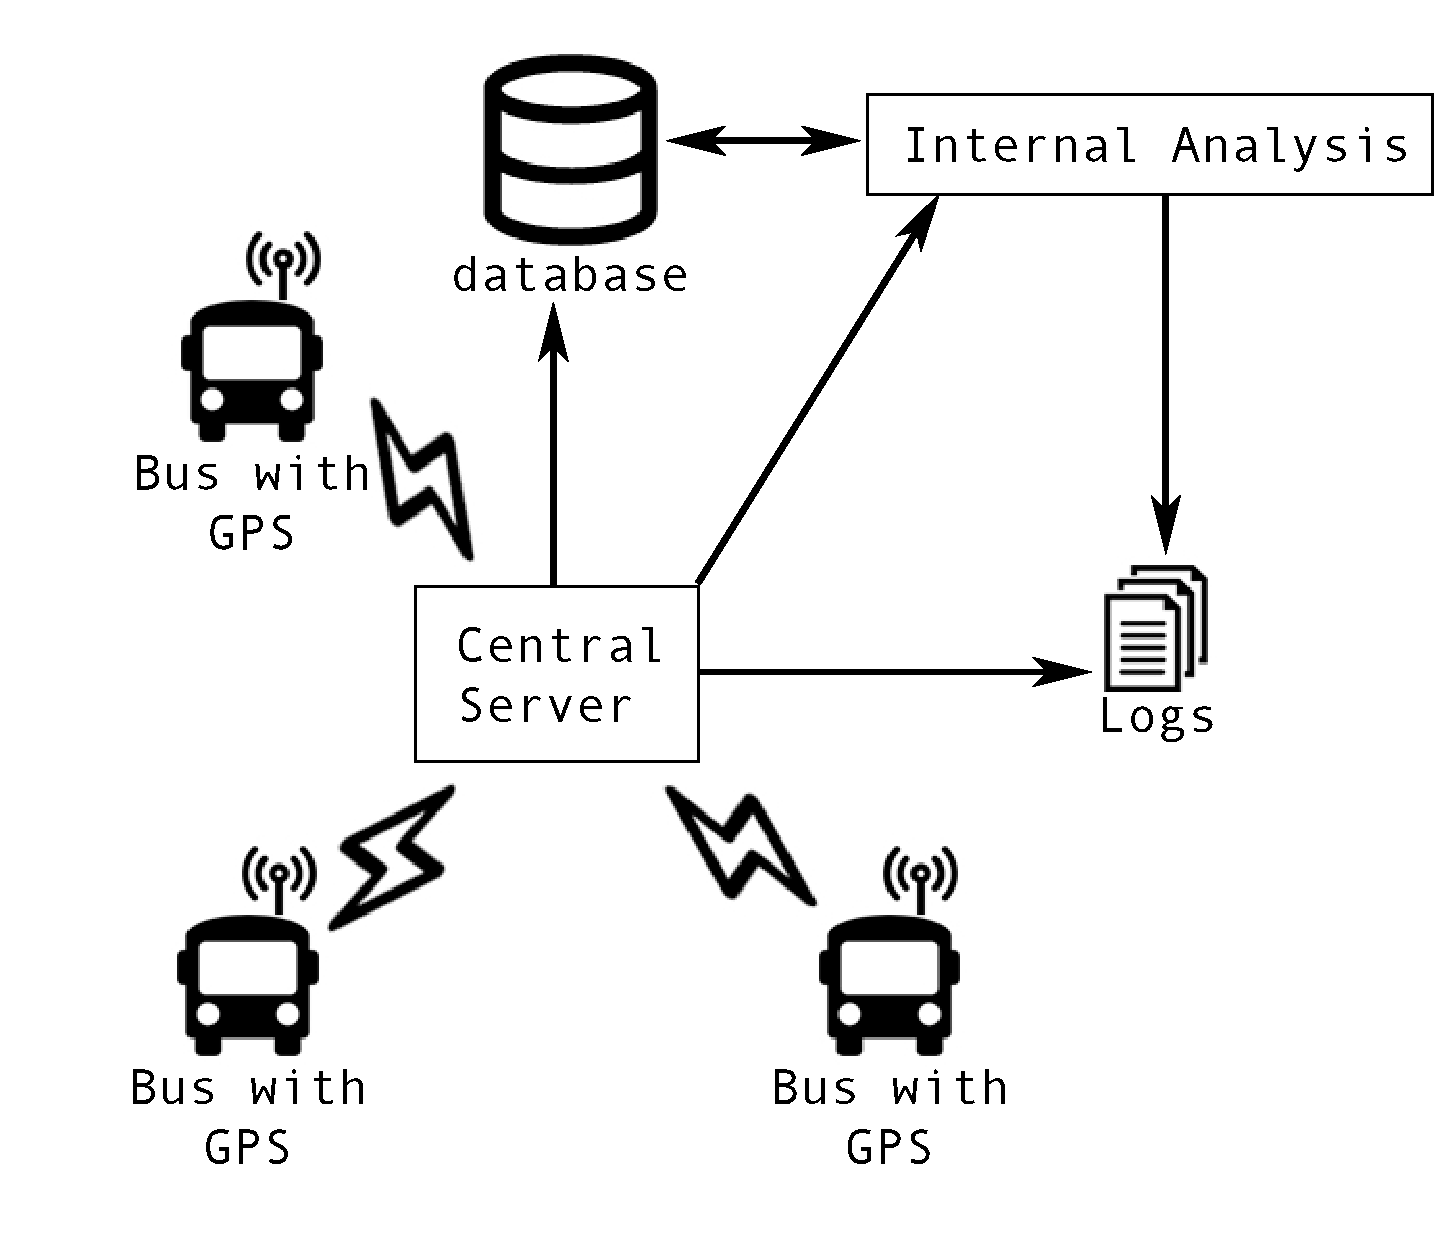
\includegraphics[width=0.75\textwidth]{figures/data-gathering}
    \caption[Simplified graph illustrating the data gathering process]
    {\small Simplified graph illustrating the data gathering process. 
    Each bus is equipped with a GPS sensor and transmits its position to a central server, which is propagated to a database.
    The dataset used in this thesis project is a collection of logs, where each log is a collection of events.
    The logs serve as a historical timeline of all events occurring at the central server.
    Examples of events occurring are the central server receiving the GPS position of a bus or events produced by the internal analysis component.}
    \label{fig:data-gathering}
\end{figure}

Figure \ref{fig:data-gathering} illustrates the procedure.
The collection of logs is the dataset used in this thesis project.
The logs contain the GPS data from the buses and also events created by the internal analysis (IA) component in the system.
The precise implementation of the IA component is unknown.

\begin{figure}[ht!]
    \centering
    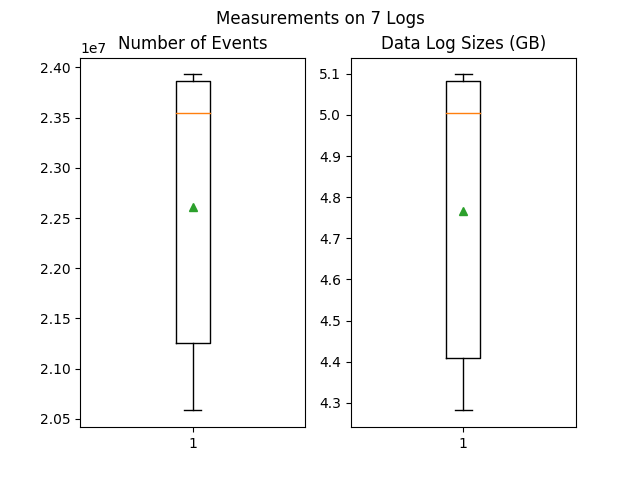
\includegraphics[width=0.7\textwidth]{figures/log_sizes}
    \caption[Average size of logs]
    {\small Average size of logs.
    Measurements are made on 7 logs (days) in the dataset.
    Naturally, there is a relationship between the number of events in a log and the size of the log.}
    The orange bar is the median, while the green triangle is the mean value.
    \label{fig:log-sizes}
\end{figure}

\section{Structure} \label{sec:data-structure}
A document in the dataset is made up of a large number of events representing a single day.
A single day typically contains about 23.5 million events, as shown in Figure \ref{fig:log-sizes}.
The orange bar is the median value, while the green triangle is the mean value.
This shows that there are a few cases where the number of events in a log are much fewer compared to the other log files.
Each event is represented by a single line of text.
An event can be split into two parts: a header and a body.
There are different types of events reported during the span of a single day.
Each type has its own header and body structure.

\subsection{Event Example}

\begin{figure}[t!]
    \centering
    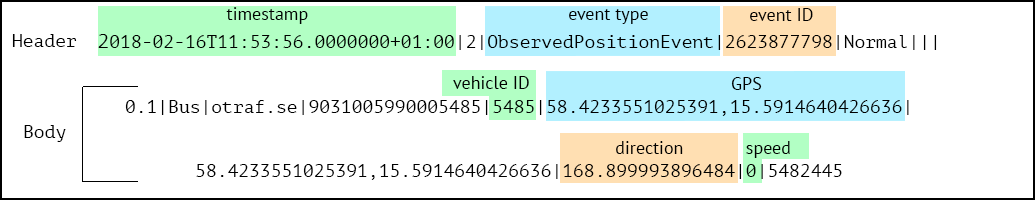
\includegraphics[width=\textwidth]{figures/data-example-1}
    \caption[Example of a raw \texttt{ObservedPositionEvent} entry]
    {\small Example of a raw \texttt{ObservedPositionEvent} entry.
    The header and the body are separated by \texttt{|||}.
    Each parameter in the header and body is separated by a single \texttt{|}.
    Key parameters for the \texttt{ObservedPositionEvent} event type is highlighted.}
    \label{fig:data-ex-1}
\end{figure}

Figure \ref{fig:data-ex-1} illustrates an event of the type \texttt{ObservedPositionEvent}.
The header is defined as all the parameters before the \texttt{|||} separator.
All the parameters after the separator are defined as the body of the event.
In this example the header and body contain seven key parameters: 
\begin{itemize}
    \item \textit{Timestamp:} A timestamp (\texttt{2018-02-16T11:53:56.0000000+01:00}), which is the timestamp from the system running on the bus.
    \item \textit{Event Type:} The event type (\texttt{ObservedPositionEvent}).
    \item \textit{Event ID:} The event id (\texttt{2623877798}). This is a number set by the system responsible for collecting the data from all buses.
    It is incremented for every event added to the log by either the database system or the IA component in Figure \ref{fig:data-gathering}.
    \item \textit{Vehicle ID:} Unique ID for the bus transmitting its position.
    \item \textit{GPS:} The GPS position of the bus in latitude and longitude.
    \item \textit{Direction:} The angle of rotation of the bus, in degrees.
    \item \textit{Speed:} The current speed of the bus, in metres per second.
\end{itemize}

\subsection{Event Types}
The dataset contains 22 unique event types.
Figure \ref{fig:types-barplot} visualises the distribution of event types for an arbitrary day in the dataset.
Only event types from buses are visualised, events from trains are discarded.
The figure only gives an indication of what the true distribution can be, as it is computationally expensive to calculate the true distribution for the given dataset, due to its size.
Knowledge about the true distribution is not required in order to reason about the event types.
As the figure shows, the majority of events that occur are of the type \texttt{ObservedPositionEvent}, which is the event containing an updated GPS position for a vehicle.

\begin{figure}[t!]
    \centering
    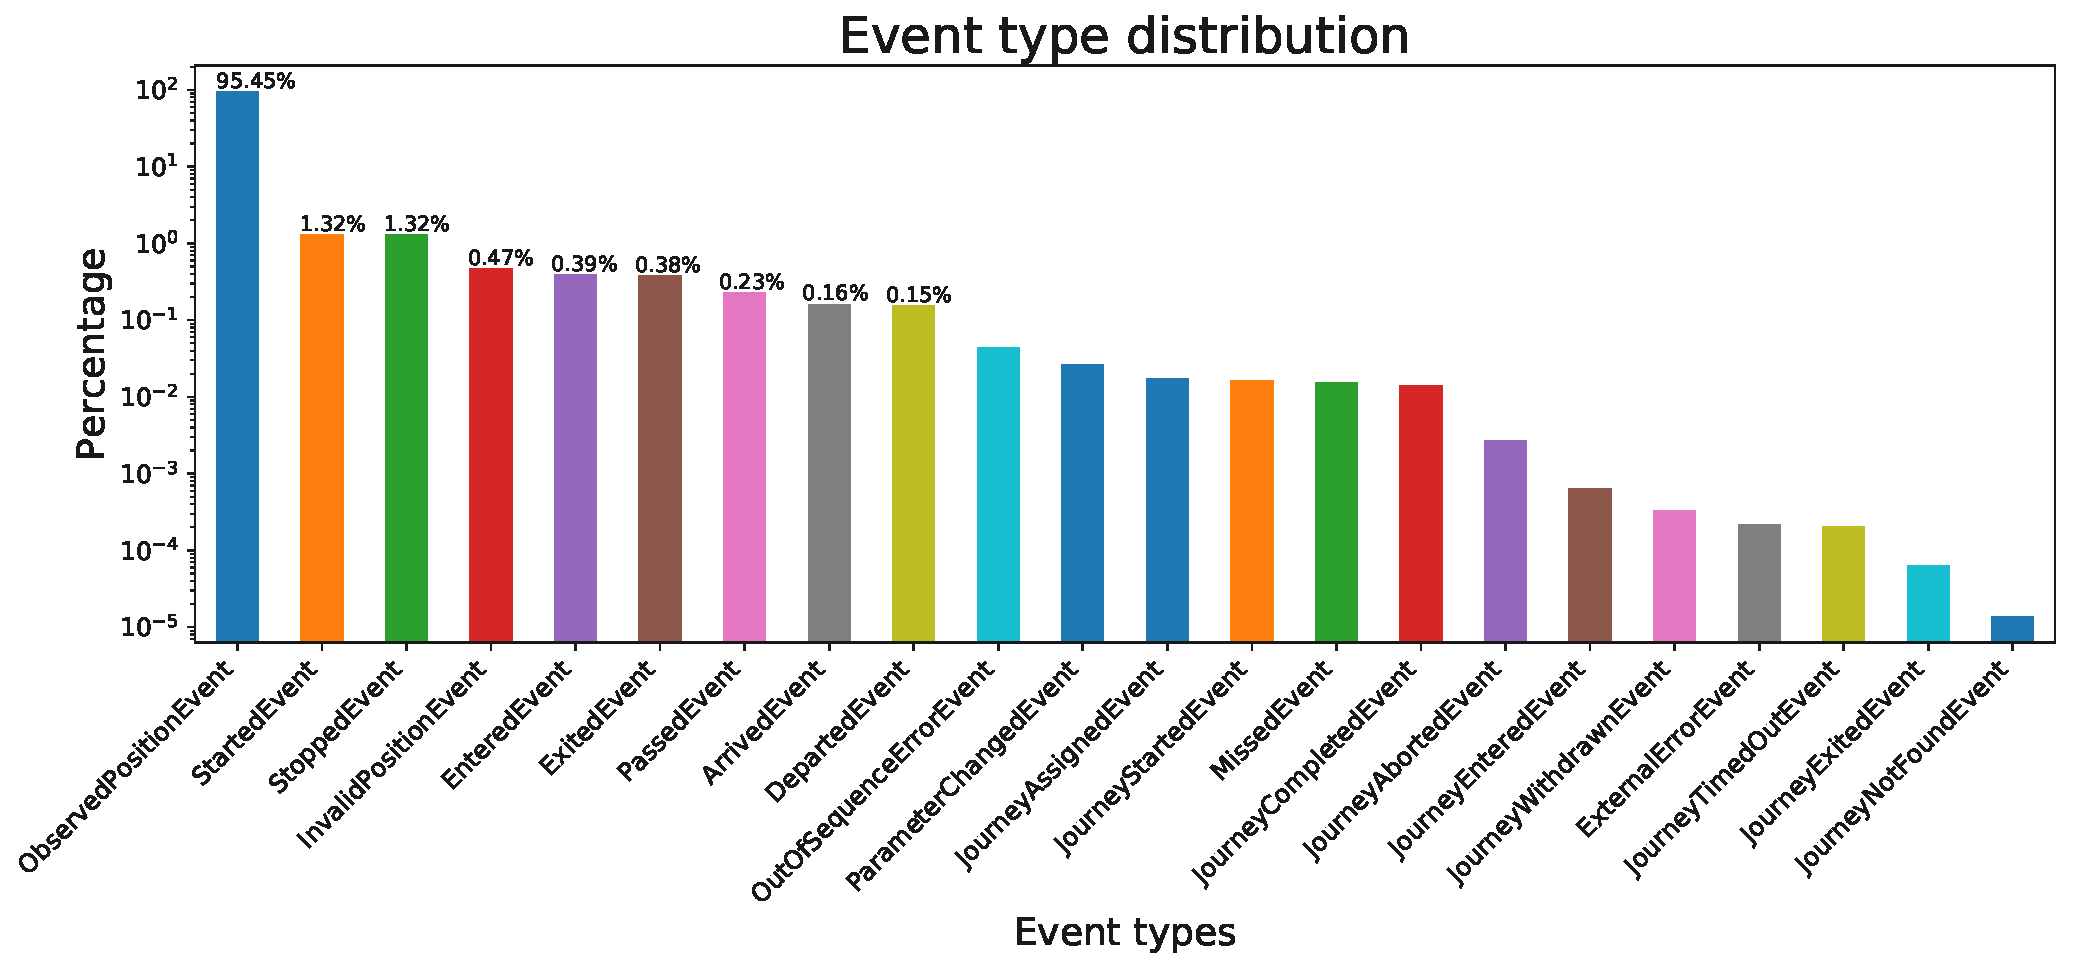
\includegraphics[width=\textwidth]{figures/types_barplot}
    \caption[The distribution of event types for an arbitrary day in the dataset]
    {\small The distribution of event types for an arbitrary day in the dataset.}
    \label{fig:types-barplot}
\end{figure}

Of the 20 event types available in the dataset, this thesis project only uses 12.
The events used are chosen by analysing the log for a single day in great detail.
Event types which occur rarely and seemingly at random are discarded, as no use can be determined for them within the scope of this thesis.
For example, the \texttt{InvalidPositionEvent} type only contains the GPS position of the vehicle.
The \texttt{ObservedPositionEvent} type also contains the \textit{Speed} and \textit{Direction} parameters.
All of the \texttt{InvalidPositionEvent}s events have the same coordinates.
In this thesis project the \texttt{InvalidPositionEvent} type is discarded, due to the missing parameters and static GPS position.

The 12 event types used in this thesis project are:
\begin{itemize}
    \item \texttt{ObservedPositionEvent}:
    This event type contains the information highlighted in Figure \ref{fig:data-ex-1}.
    It is the most prevalent event type in the provided dataset.
    This event type is contextless, as it contains no information about which public transportation line the vehicle is currently serving, if any. 
    
    \item \texttt{StartedEvent} and \texttt{StoppedEvent}:
    These two event types provide context to a sequence of observed position events.
    They denote when the vehicle has started or stopped moving, respectively.
    For example, they can be used to identify road intersections, bus stops, traffic or driver breaks.
    
    \item \texttt{EnteredEvent} and \texttt{ExitedEvent}:
    These two event types are used by the IA component to identify bus stops.
    The \texttt{EnteredEvent} is produced by the system when the vehicle is within a certain predefined distance of a bus stop.
    The \texttt{ExitedEvent} is similarly produced when the vehicle leaves the predefined distance of the bus stop.
    These event types can, for example, be used in an algorithm which improves the bus stop detection.
    
    \item \texttt{PassedEvent}, \texttt{ArrivedEvent}, and \texttt{DepartedEvent}:
    These three event types are used to provide information regarding which bus stop a particular bus is at.
    The \texttt{PassedEvent} type denotes when a particular bus, serving a specific public transportation line, passed a bus line stop.
    It contains information about the predefined position of the stop, the public transportation line the particular bus is currently serving and the time of the passing.
    Similarly, the \texttt{ArrivedEvent} and \texttt{DepartedEvent} types denote when a particular bus arrives at or departs from a particular bus stop.
    These event types provide context to the observed positions.
    In this thesis project they are used to group a sequence of observed positions into a segment between two stops for a particular bus line.
    
    \item \texttt{ParameterChangedEvent}:  
    The \texttt{ParameterChangedEvent} type is the most dynamic event type in the data set.
    For example, it can be used to inform the system when the doors on a particular bus open or close or when a bus changes journeys.
    In this thesis project it is only used to identify bus lines and give context to observed positions.
    
    \item \texttt{JourneyStartedEvent} and \texttt{JourneyCompletedEvent}: \newline
    The \texttt{JourneyStartedEvent} type is produced by the IA component when a bus has reached the starting bus stop of a bus line.
    The \texttt{JourneyCompletedEvent} event type is produced when the bus has reached the final bus stop of a bus line.

    \item \texttt{JourneyAssignedEvent}:
    This event type is in most cases accompanied by a \texttt{ParameterChangedEvent} to denote when a bus changes its journey.
    It contains the time of the assignment, the position of the bus and the bus line the bus is assigned.
    The information is thus similar to the \texttt{ParameterChangedEvent}.
\end{itemize}

\section{Dataset Pre-Study}
The dataset pre-study is conducted after the basic characteristics are identified.
It analyses the dataset in greater depth, identifying interesting scenarios that occurs in the data.
The analysis is conducted by manually parsing the data.
This manual task uses EDA methods to simplify the process; the focus is put on visualising the data in order to detect patterns and outliers.
All events during an arbitrary day are initially used for this task.
Anomalies that occurred are isolated and categorised by applying the rationale behind the binary search algorithm.
The log is divided in two equal halves in order to see which half inhibits the anomalies.
The procedure is repeated as long as anomalies are present.
This halves the search space at each iteration, as long as anomalies are not present in both halves.
If an anomaly is missing from both halves it is an indication that the anomaly occurs by combining the events around the split.

The search is more complex than one simple binary search algorithm run, as anomalies can occur in both splits.
If anomalies are present in both splits, the split intervals are saved and then the search proceeds in one of the splits.
When the search exhausts the arbitrarily chosen split, it starts searching the other split using the saved interval.
The method can thus be seen as a binary search algorithm which branches and starts another binary search processes if anomalies are detected in both splits. 

Three interesting scenarios are identified in the dataset pre-study: human error induced early stopping, imprecise algorithms causing final bus stops to be missed, and self-overlaps.

\subsection{Human Error: Early Stopping}
Figures \ref{fig:human-error-early-stopping-1} and \ref{fig:human-error-early-stopping-2} illustrate two scenarios when the \texttt{JourneyCompletedEvent} type for a started journey is missing.
In Figure \ref{fig:human-error-early-stopping-1}, the bus driver is supposed to follow the red line and visit the three markers in order to complete the journey for a particular line.
Instead, the bus follows the green line and the three markers are skipped.
In Figure \ref{fig:human-error-early-stopping-2}, the bus drives along the planned path (the green line).
When the bus reaches the crossing marked by the arrow, the bus turns and drives along the blue line instead of following the planned route (the red dashed line).
In both these real-world examples, the bus drivers ignore the last few bus stops of the bus lines.

The IA component never deems the journey as completed in these scenarios, which results in the \texttt{JourneyCompletedEvent} type never being produced.
This scenario is easy to detect in historical data, but in real-time certain assumptions need to be made.
For example, if the journey is compared with an average journey, the anomaly can be detected early.
However, it is uncertain if the anomaly is due to a journey being stopped early or if the bus driver took a wrong turn on the highway.
A time constraint threshold can be introduced to the system in order to separate these two cases.
In the case of a wrong turn, the bus eventually converges to the average journey, while in the early-stopping scenario the journey most likely never converges.

\begin{figure}[!ht]
    \centering
    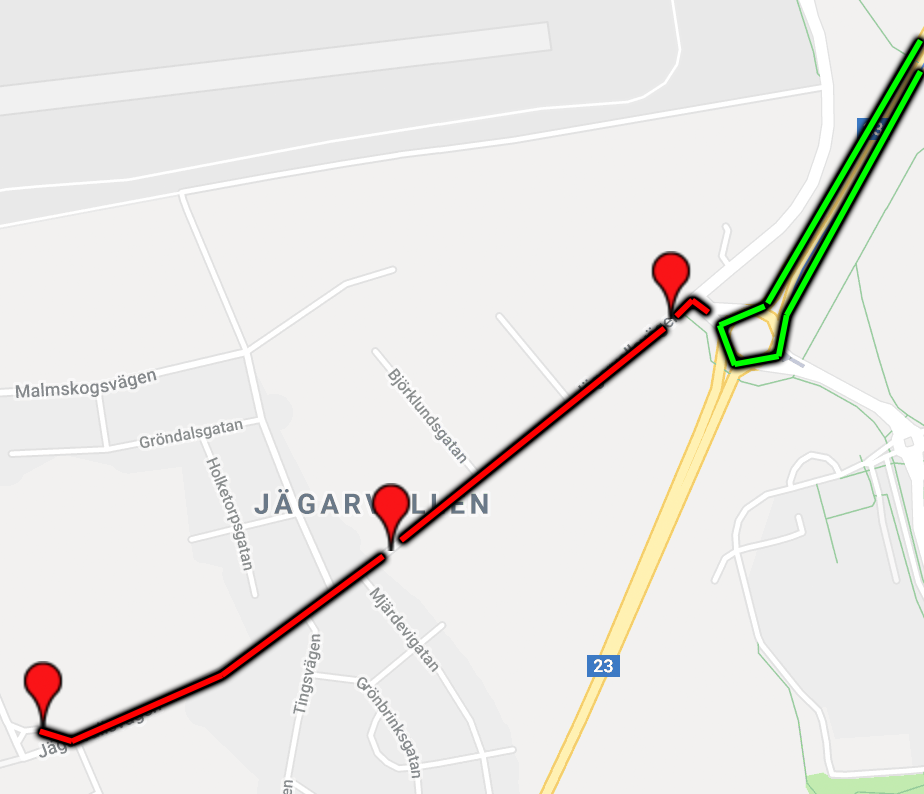
\includegraphics[width=0.7\textwidth]{figures/edge_case_early_quit}
    \caption[Example of early stopping in a journey]
    {\small Example of early stopping in a journey.
    The three markers are the final three stops of a particular bus line.
    The green line is the route the bus drives.
    Instead of following the planned, red route of the bus line, the final three stops are skipped.
    This results in the journey never being deemed completed.}
    \label{fig:human-error-early-stopping-1}
\end{figure}

\begin{figure}[!ht]
        \centering
        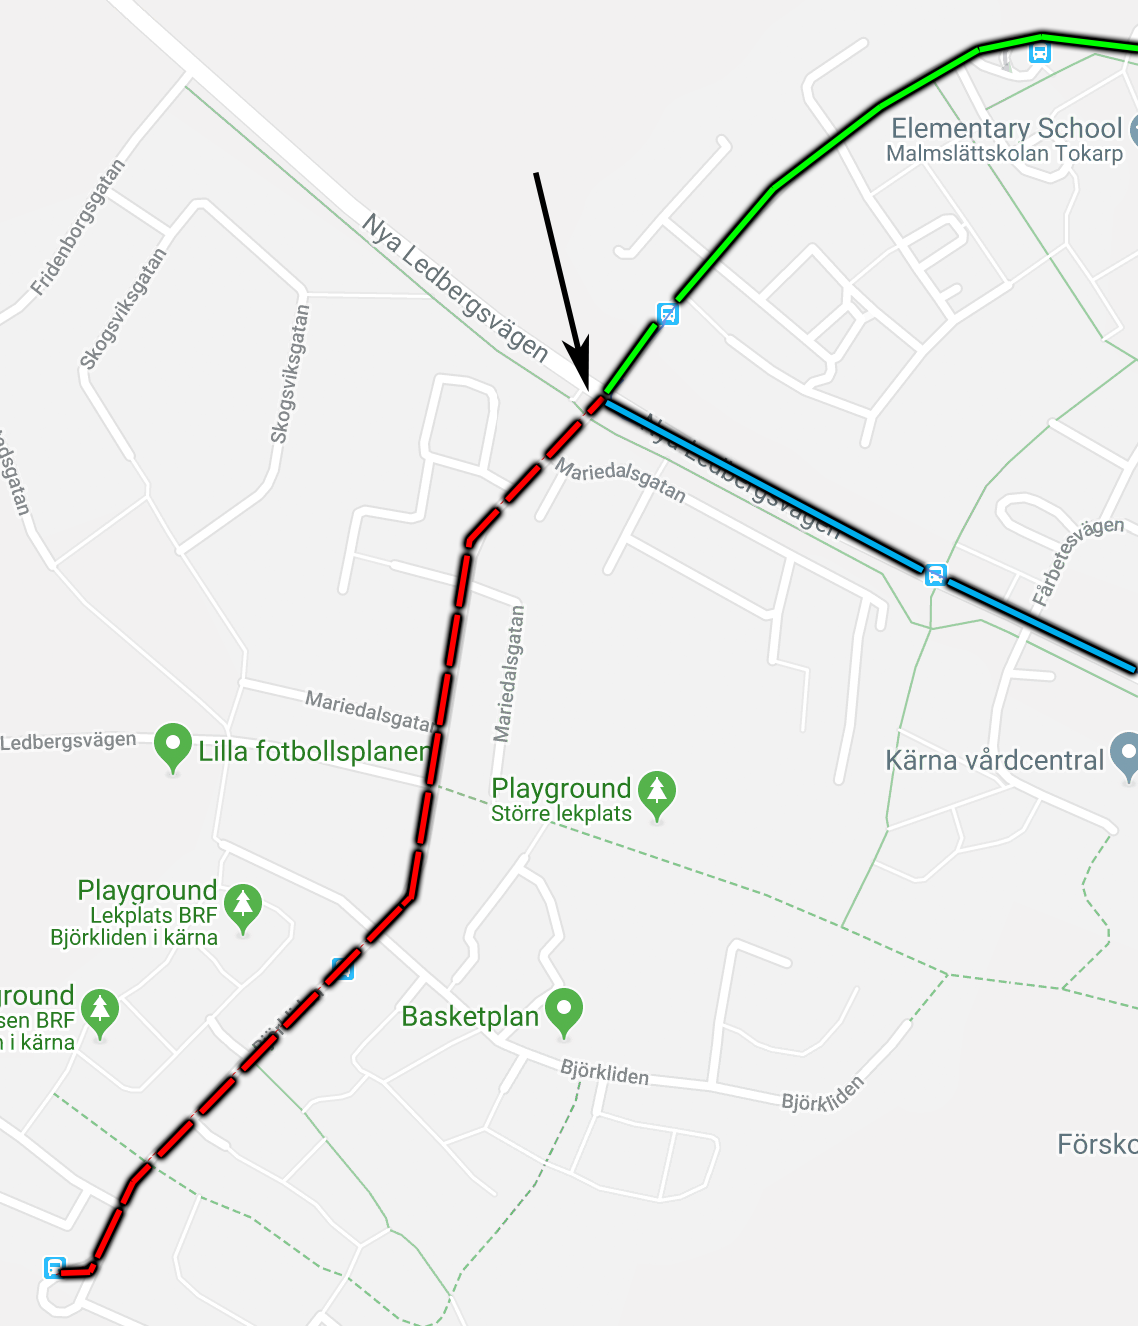
\includegraphics[width=0.7\textwidth]{figures/lazy_driver_2}
        \caption[Another example of early stopping in a journey]
        {\small Another example of early stopping in a journey.
        The bus drives on the green line and reaches the crossing marked by the arrow.
        The planned route for the bus line is to follow the red dashed line.
        Instead of following the planned route, the bus drives along the blue line.
        This results in the journey never being deemed completed, creating an erroneous ordering of contextual events (\texttt{JourneyCompletedEvent} never received).}
        \label{fig:human-error-early-stopping-2}
\end{figure}

\begin{figure}[!ht]
    \centering
    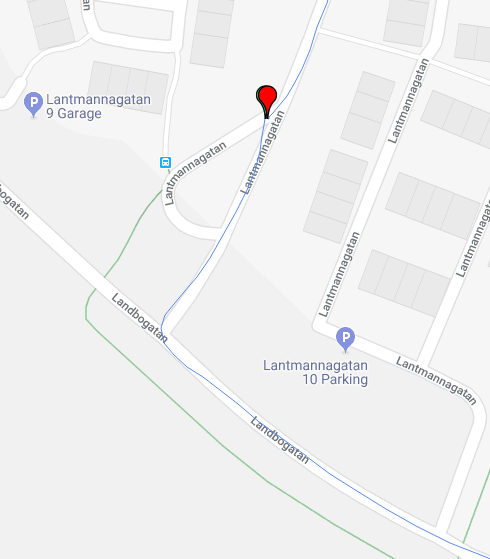
\includegraphics[width=0.6\textwidth]{figures/stopped_before_end}
    \caption[Real-world example of a bus driver stopping roughly 45 meters before reaching the final bus stop]
    {\small Real-world example of a bus driver stopping roughly 45 meters before reaching the final bus stop.
    The final bus stop of the bus line is marked on the map by the blue bus icon (indicated by the black arrow).
    The red marker is the GPS position where the bus stopped.
    The blue line is the route the bus drives.
    The bus stops at the marker for a few minutes before it continues to the first bus stop for the next journey.
    The system does not register the bus as having passed the bus stop indicated by the black arrow.
    Thus, the system does not determine the journey as completed.
    This causes the route after the red marker to be included in the trajectory.
    The bus stop detection algorithm systematically does not identify the cases where a bus stops at a "waiting" space.}
    \label{fig:stopped-before-end}
\end{figure}

\newpage
\subsection{Imprecise Algorithms: Final Bus Stop Missed}
This scenario occurs due to a mix of imprecision in the bus stop detection algorithm and human error.
The scenario is illustrated in Figure \ref{fig:stopped-before-end}.
The bus driver completes the journey of a particular bus line and reaches the final bus stop.
However, the IA component does not detect that the bus stop has been reached.
This is due to the bus driver stopping the bus roughly 45 meters before the final bus stop.
The bus stops at the red marker for a few minutes, before it starts driving towards the first bus stop of the next planned journey.
The route after the red marker is erroneously included in the journey for the bus line, as the journey is never completed.

This systematically occurs at certain bus stops, due to there being a "waiting" space commonly used by bus drivers while waiting for a new journey to be assigned.
The scenario highlights a problem with the implemented bus stop detection algorithm.
The bus stop detection algorithm can be improved to both handle these scenarios and yield more precise bus stop detection.
An improved bus stop detection method is proposed in Chapter \ref{cha:bus-stop-detection}.

Missed final bus stops cause problems for both the data analysis and for specific applications.
For example, journeys contain more \texttt{ObservedPositionEvents} than they should, as the journeys are never deemed completed.
This results not only in journeys being discarded as erroneous, but also affects other events and the ordering of events.
The pre-processing step has to adapt to these problems, which increases the complexity of the data pre-processing.

\subsection{Self-Overlap} \label{sec:self-overlapping-trajectories}

Self-overlap causes issues when used as training data for GP models \cite{Tiger2018-gp-motion-pattern}.
Self-overlapping causes instabilities.
In the specific applications of this thesis project, self-overlapping causes problems with the trajectory forecasting.
For example, overlapped GPS positions results in ambiguous arrival time predictions.

An example of self-overlap is shown in Figure \ref{fig:self-overlap}.
Self-overlap can be detected manually by visually looking at the trajectories, which is the method used in this thesis project.
In \cite{Tiger2018-gp-motion-pattern}, an approach to handling and detecting self-overlaps is explained.
The distances between subsequent points on a latent function $f$ of the trajectory is calculated with a given resolution $\theta$.
It is possible, using this approach, to find self-overlaps down to the given resolution \cite{Tiger2018-gp-motion-pattern}.
Generally, $f$ is unknown and needs to be estimated using a GP model trained on the full trajectory \cite{Tiger2018-gp-motion-pattern}.
If the pair-wise distance between non-subsequent interpolated points is under a threshold, then the self-overlap is detected.   

\begin{figure}[t!]
    \centering
    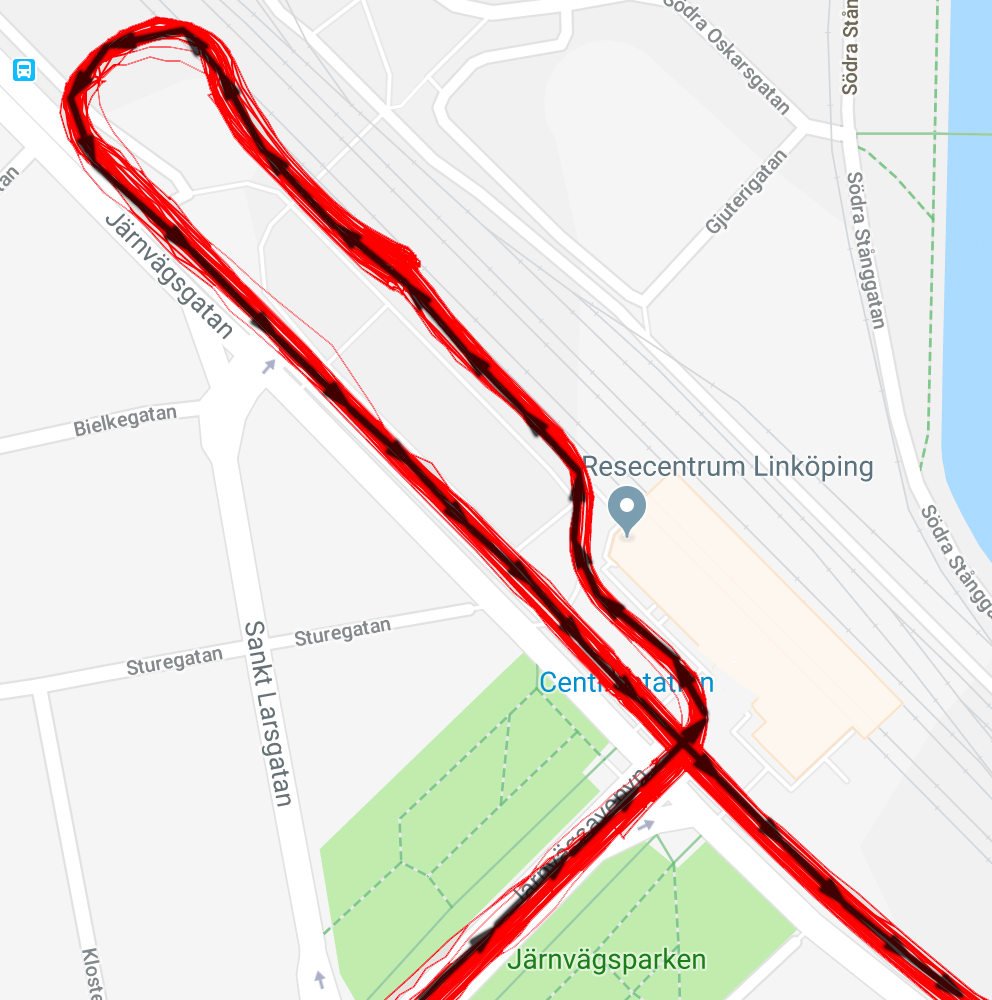
\includegraphics[width=0.6\textwidth]{figures/self-overlap}
    \caption[Example of self-overlap in a bus journey]
    {\small Example of self-overlap in a bus journey. 
    The red lines show the trajectories of the buses driving for the same bus line.}
    \label{fig:self-overlap}
\end{figure}

\section{Pre-Processing Events} \label{sec:pre-process-events}
The first step deemed necessary in order to use the data in the provided dataset is to transform it from strings to objects with attributes.
Figure \ref{fig:data-ex-1} visualises which attributes an \texttt{ObservedPositionEvent} object contains.
Similar structures are created for each of the mentioned event types.

During this pre-process step all the events from a vehicle type other than "Bus" are ignored.
A \textit{geo-fence} is applied in order to facilitate and support manual inspection and visualisation of the data in the dataset.
A geo-fence is a virtual polygon which establishes a virtual perimeter for a real-world geographical area.
The geo-fence applied in this thesis project is shown in Figure \ref{fig:geo-fence}.

\begin{figure}[t]
    \centering
    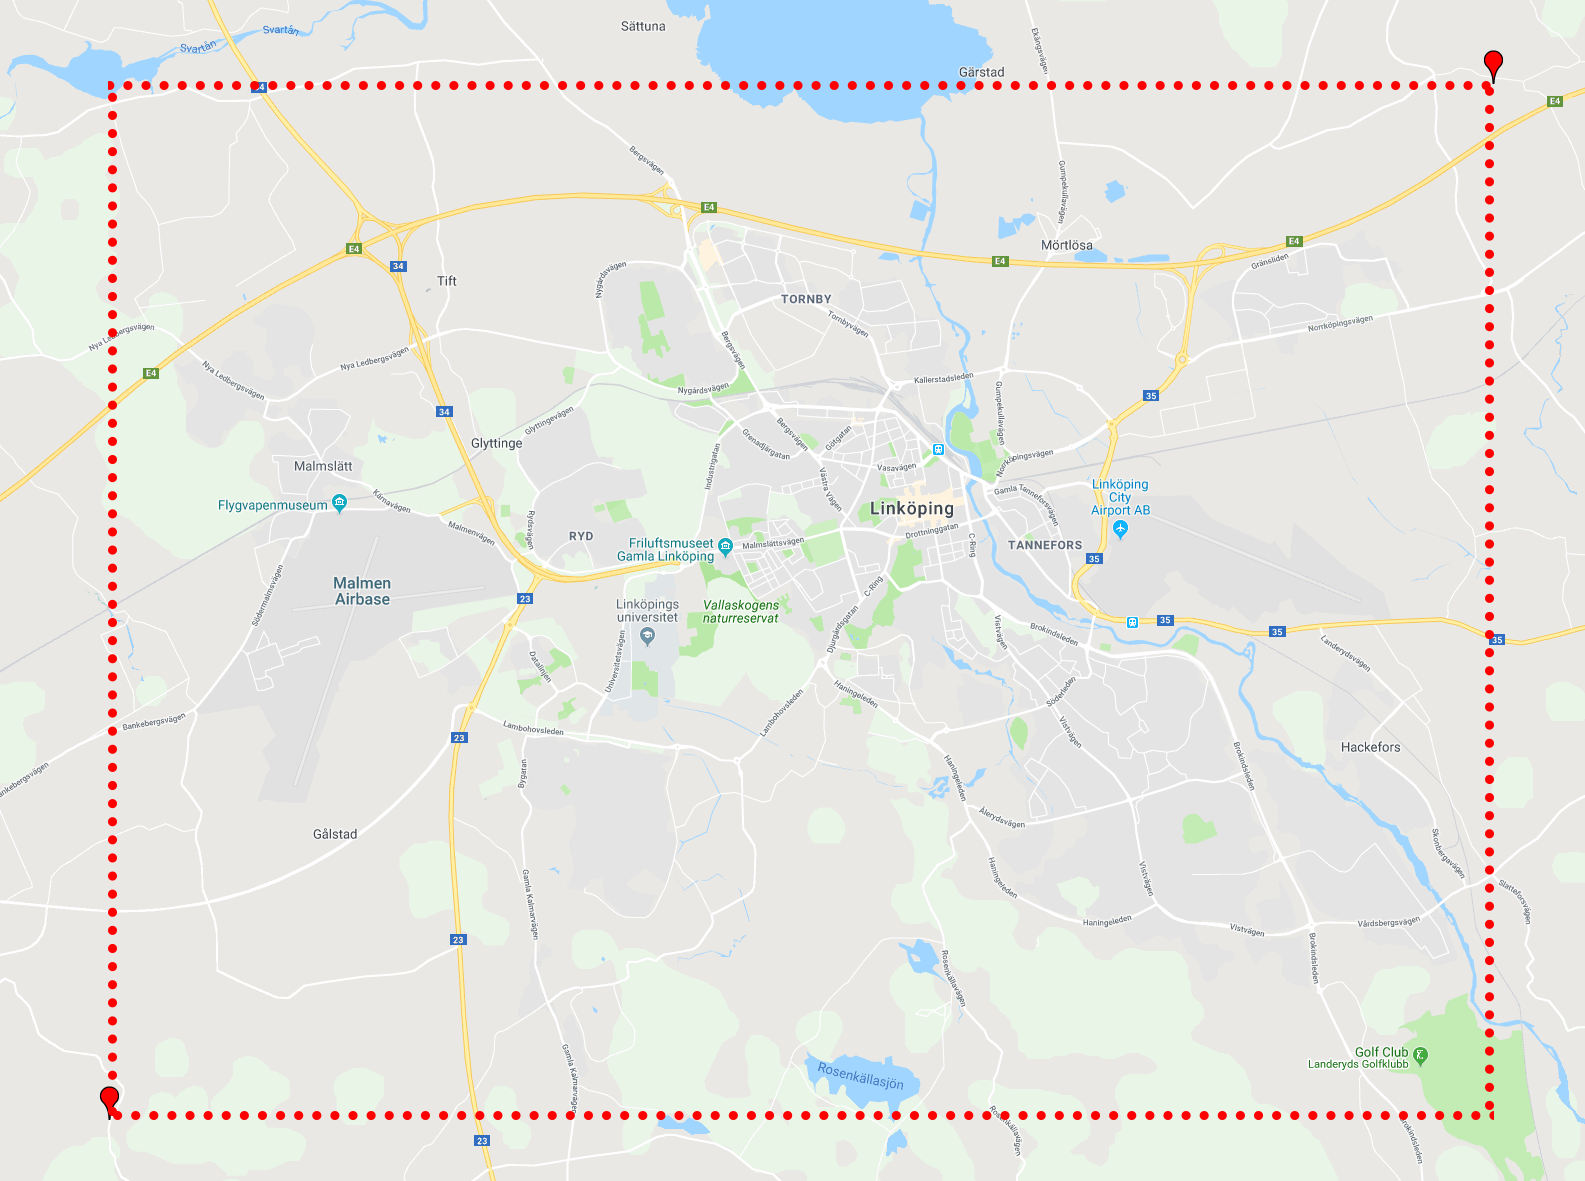
\includegraphics[width=\textwidth]{figures/geofencing_linkoping}
    \caption[A geo-fence is constructed to filter out events occurring outside the virtual perimeter]
    {\small A geo-fence is constructed to filter out events occurring outside the virtual perimeter.
    The two red markers create a rectangular boundary, which is illustrated with the red-dotted line.
    The geographical area is the city of Linköping.}
    \label{fig:geo-fence}
\end{figure}

\begin{figure}[t]
    \centering
    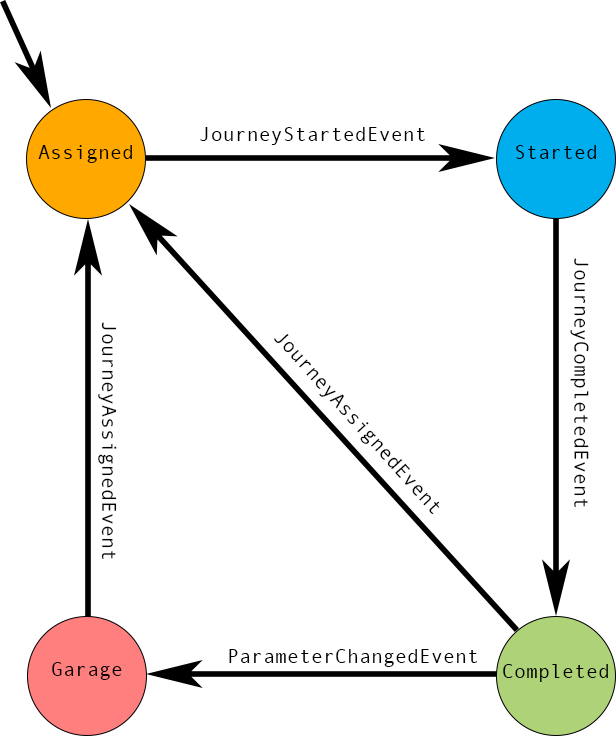
\includegraphics[width=0.7\textwidth]{figures/context-state-machine}
    \caption[Finite-state machine providing context to \texttt{ObservedPositionEvent}s]
    {\small Finite-state machine providing context to \texttt{ObservedPositionEvent}s. 
    The constructed FSM is simplified to illustrate the best-case scenario.
    The "Assigned" state is the starting state.
    \texttt{ObservedPositionEvent}s are assigned to the current FSM state.
    }
    \label{fig:context-state-machine}
\end{figure}

After the parsing and filtering step the idea is to provide context to \texttt{ObservedPositionEvent}s.
Only using this one contextless event type greatly reduces the span of potential problems one can solve with the provided dataset.
Context is provided by constructing a FSM.

\subsection{Context-Providing Finite-State Machine}
The context-providing FSM constructed in this thesis project is shown in Figure \ref{fig:context-state-machine}.
The shown state machine is illustrating the best-case scenario, when the actual order of events is equal to the logical ordering of events, see Figure \ref{fig:assigned-before-completed-working} for a real-world example.
However, this is not always the case when working with real-world data, as shown in Figures \ref{fig:assigned-before-completed-long} and \ref{fig:assigned-before-completed}.
Occasionally the timing of events gets mixed up, e.g. a bus in the "Started" state receives a \texttt{JourneyAssignedEvent} before it receives a \texttt{JourneyCompletedEvent}.
This ordering breaks the logical ordering of events: a journey needs to be completed before a new one can assigned.

\begin{figure}[t]
    \centering
    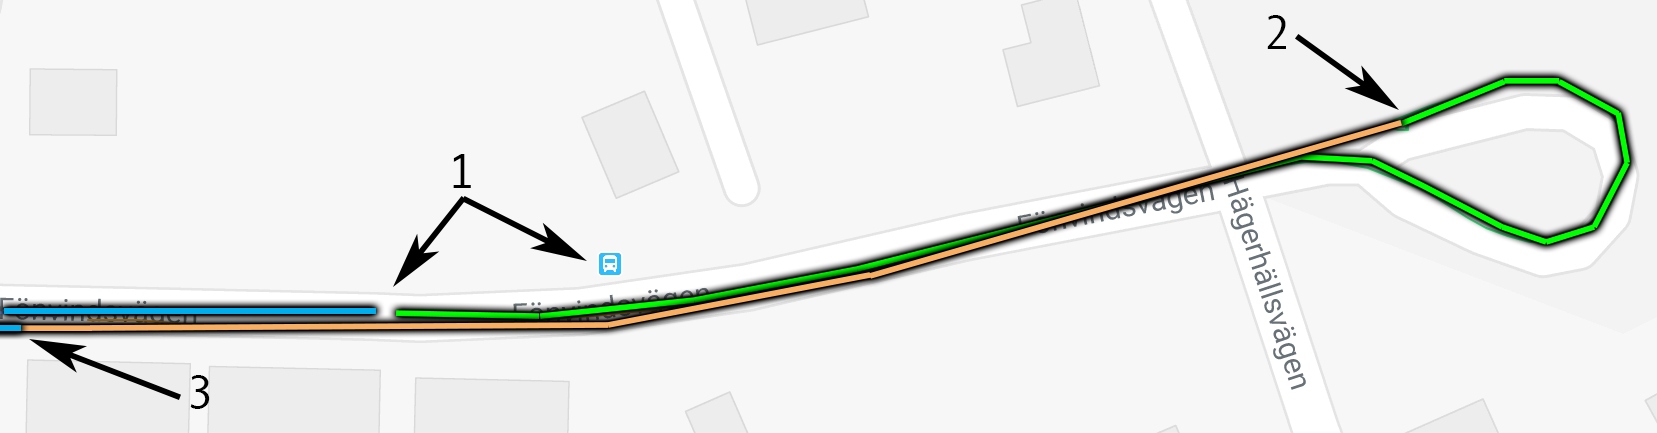
\includegraphics[width=1\textwidth]{figures/assigned_completed_working}
    \caption[Real-world scenario illustrating when events occur in a logical ordering]
    {\small Real-world scenario illustrating when events occur in a logical ordering.
    The blue line is \texttt{ObservedPositionEvent}s in the "Started" state.
    Upon reaching the final bus stop for the line the state changes to "Completed" (1).
    The \texttt{ObservedPositionEvent}s for this state is drawn with a green line to denote the "Completed" state.
    The bus turns around and stops for a period of time until a new bus line is assigned to it (2).
    In this particular scenario, the bus is assigned the same bus line number, but in the opposite direction.
    The orange line denotes the \texttt{ObservedPositionEvent}s in the "Assigned" state.
    Shortly after passing the first bus stop the orange line changes to blue (3), which denotes the "Started" state.}
    \label{fig:assigned-before-completed-working}
\end{figure}

\begin{figure}[t]
    \centering
    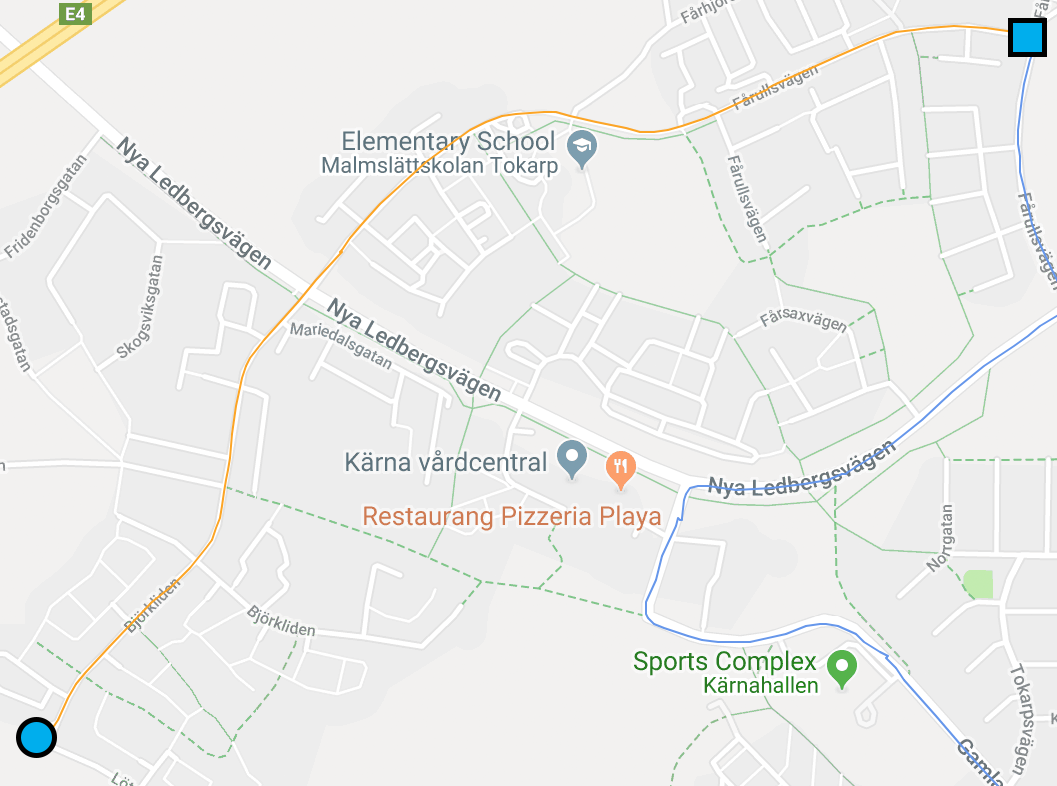
\includegraphics[width=0.6\textwidth]{figures/assigned_completed_problem_long}
    \caption[Example of early stopping in a journey]
    {\small Example of early stopping in a journey.
    The bus is assigned a new bus line long before reaching the final bus stop.
    The final bus stop is marked with a circle.
    The rectangle marks the position of the bus when it is assigned a new bus line.
    The last part of the journey (the path between the rectangle and the circle) is thus assigned to a new state "Assigned", instead of the actual, logical state "Started".}
    \label{fig:assigned-before-completed-long}
\end{figure}

\begin{figure}[t]
    \centering
    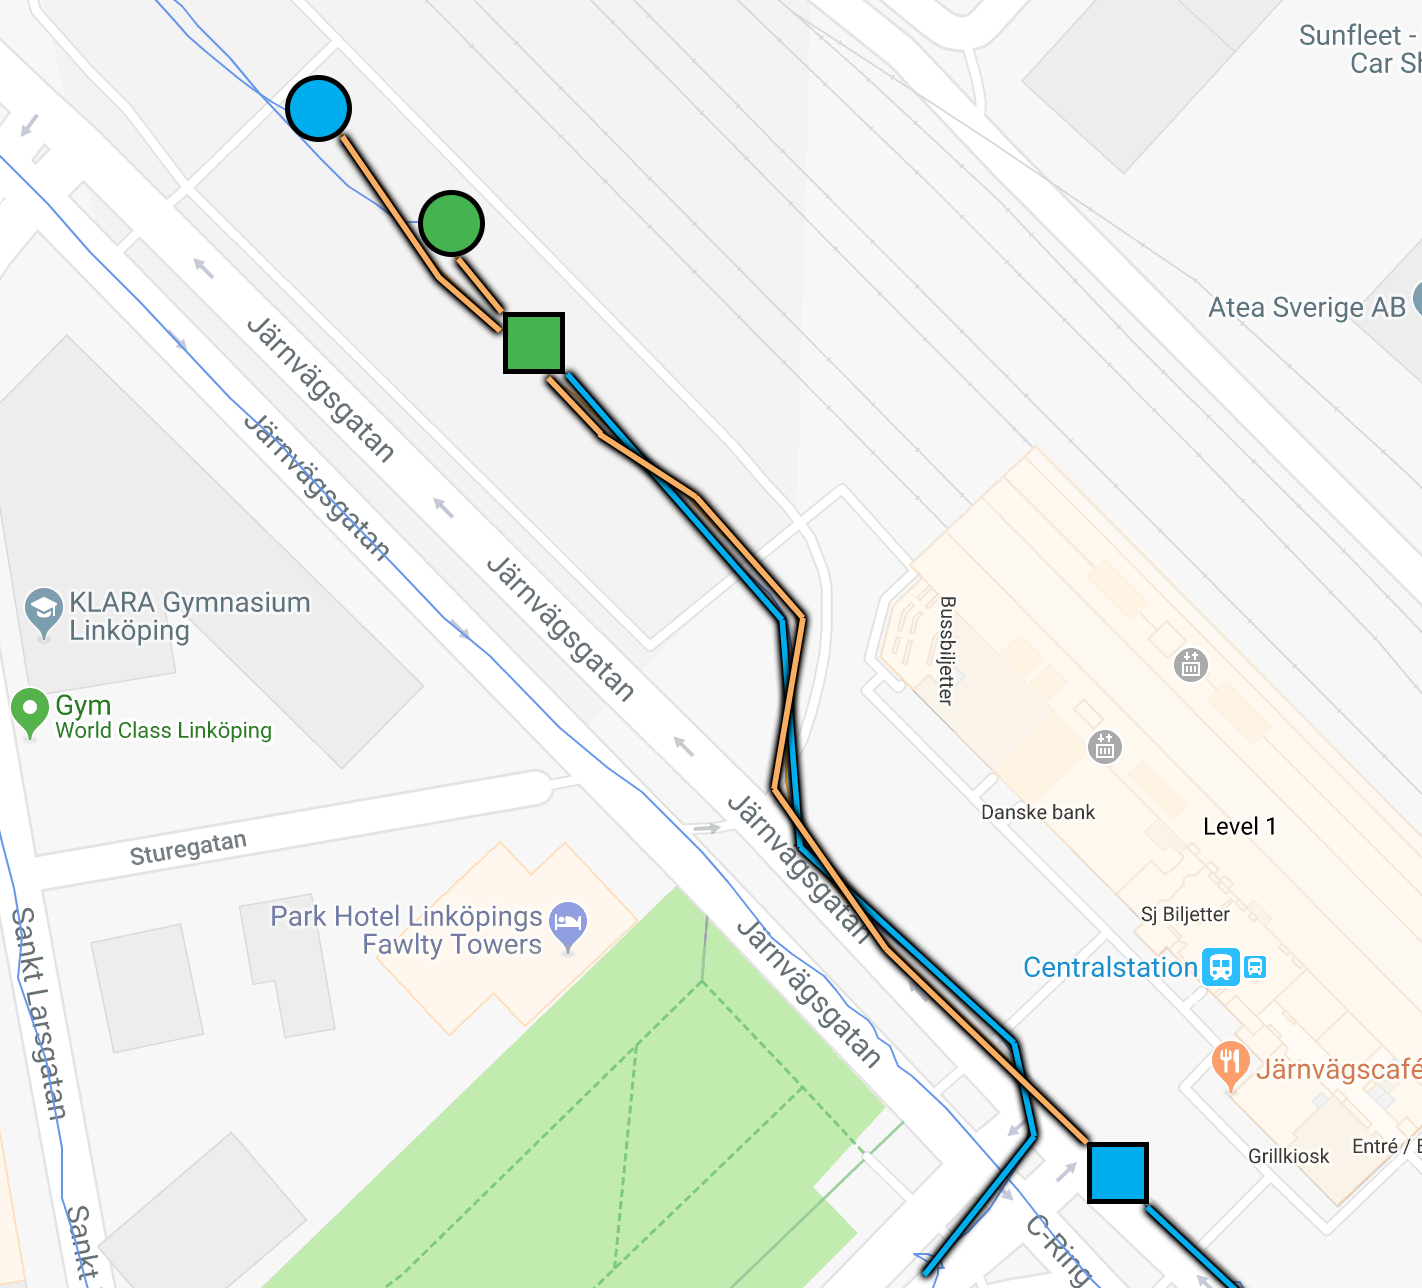
\includegraphics[width=0.6\textwidth]{figures/assigned_completed_problem}
    \caption[Another example of early stopping in a journey]
    {\small Another example of early stopping in a journey.
    The two circles (green and blue) denote the final bus stops for the respective bus lines.
    One of the buses is assigned a new bus line at the blue rectangle in the bottom-right corner, long before reaching the final bus stop.
    The other bus is assigned a new bus line at the green rectangle, which is closer to the final bus stops.
    This example demonstrates that the assignment to a new bus line is independent of the distance to the final bus stop.}
    \label{fig:assigned-before-completed}
\end{figure}

The problem is partly solved by changing the ordering of events from \textit{Timestamp} to \textit{Event ID}.
This is a feasible approach when the data is batched into separate files, where one file is a full day of events.
Unfortunately, this approach does not work when dealing with streamed real-time data, as the ordering cannot be changed without introducing a buffer.
The context-providing FSM is slightly altered in order to support the processing of streamed real-time data.
Another motivation behind the change is to remove the assumption that the sequence of \textit{Event ID}s is always correct. 
The \texttt{ObservedPositionEvent}s are instead placed in a temporary buffer once an anomaly is detected in the event ordering.
For example, if a new \texttt{JourneyAssignedEvent} is received before the supposed \texttt{JourneyCompletedEvent} and the system is in the "Started" state.
Once the \texttt{JourneyCompletedEvent} type is received, after some delay, the data in the buffer is retroactively added to the "Started" state.
The "Started" state then correctly contains all \texttt{ObservedPositionEvent}s received from the starting bus stop to the final bus stop.
However, it is not always the case that the \texttt{JourneyCompletedEvent} type is contained in the journey.
Occasionally, the type is missing from the sequence of events due to either human errors or imprecise algorithms in the IA component.
These scenarios can easily be detected by utilising the context-providing FSM with the added buffer extension.

\subsection{Bus Stops}
Using the FSM provides context to the \texttt{ObservedPositionEvent} types.
The states introduced yield a simple way to visualise contextual paths, e.g., actual journeys for a particular bus line or the path a bus drives to start a journey under a new bus line number.
However, the context-providing FSM solution described does not handle events about a bus arriving, departing or passing a bus stop on the journey.
Handling this type of data is a critical step in detecting imprecisions in the bus stop detection algorithm or early stopping due to human error.
The "Started" state in the FSM can be extended to not only include \texttt{ObservedPositionEvent} types, but also \texttt{ArrivedEvent}, \texttt{DepartedEvent}, and \texttt{PassedEvent} types.
A missed final bus stop can then, for example, be identified by looking at all the bus stops added to the "Started" state for that journey and compare them to the bus stops in other journeys for that particular bus line.
Extending the FSM to handle the bus stop data causes the complexity of the FSM to increase.

An alternative approach is implemented instead, as the existing context-providing FSM can easily be verified to produce correct output.
The approach extracts all events of the types \texttt{StartedEvent}, \texttt{StoppedEvent}, \texttt{PassedEvent}, \texttt{ArrivedEvent}, and \texttt{DepartedEvent} for each specific \textit{Vehicle ID}.
These events are then paired with the journeys for each respective \textit{Vehicle ID}.
Any events of the type \texttt{StartedEvent} or \texttt{StoppedEvent} occurring before the first \texttt{ObservedPositionEvent} of the journey are discarded.
Events of the type \texttt{PassedEvent}, \texttt{ArrivedEvent} or \texttt{DepartedEvent} are included in the journey if they occur within a specific period of time to the first \texttt{ObservedPositionEvent}. 
When all \texttt{ObservedPositionEvent}s of a journey are processed, the procedure continues with the next journey.
The set of extracted events thus naturally reduces in size for each journey processed.
Events occurring in-between journeys are discarded.
When adding a bus stop to the journey, the name of the bus stop is also added to a separate array, in order to simplify the process of detecting erroneous journeys.

\subsection{Results}
The result of the pre-processing step is a collection of journeys for each bus line.
A journey consists of all the \texttt{ObservedPositionEvent}s sent by the bus while the FSM is in the "Started" state and all the bus stops the bus arrived at, departed from or passed by.
It also contains all the stops and starts made by the bus during the journey.
Erroneous event type ordering is solved by sorting the events based on \textit{Event ID} and using a buffer to retroactively add \texttt{ObservedPositionEvent} in the "Assigned" state to the "Started" state in the case of an early journey assignment.
Journeys with early stopping or missed final bus stops are still prevalent in the collection of journeys.
These can be detected by analysing the bus stops registered during a journey.
In this thesis, the erroneous journeys are only marked as anomalies and discarded.
An index-tree is constructed to quickly access all journeys for a bus with a particular \textit{Vehicle ID}.
A number of high-level problems can now be formulated by using the result from the pre-processing steps.

\subsection{Discussion}
The erroneous journeys are only marked as anomalies and discarded in this thesis.
The fraction of erroneous journeys can be calculated and used as a baseline when comparing an improved bus stop detection method with the existing one.
Erroneous journeys can be categorised based on the error in the journey, e.g., a missed starting bus stop is a different error compared to a missed final bus stop.
The categorisation of faults can provide deeper insights into the dataset.
For example, the insights can be used to improve the bus stop detection algorithm or identify journeys where a particular error occurs regularly.

\subsection{Discarded Event Types}
The discarded event types can be investigated in-depth with regard to the whole dataset and not only for an arbitrary day.
Some of the events can perhaps be used to easier detect or handle the erroneous journeys.
During the initial manual processing of the data, no use is discovered for any of the excluded event types.
This may be an indication that the rarer event types are wrongly produced by the IA component.
A more probable explanation is that the method of manually investigating the context different event types occur in is subpar and prone to human errors.
An automated approach tailored to focus on rare event types probably yields better results and a use for the discarded event types.

\subsection{Train Events}
It would be interesting to perform the same analysis done in this chapter on the data from public transportation trains.
The trains exhibit different behaviour than busses, as traffic is different and perhaps more static, with dedicated waiting tracks.

\section{Future Work}
The discarded event types should probably be explored further.
In a setup with more processing power, the requirement of a geo-fence can be removed.
Different environments can easily be analysed by allowing events from a larger geographical area.
The context-providing FSM probably has to be changed after analysing discarded event types, if any of them are deemed useful.
Perhaps a combination of discarded events can result in a simplification to be possible in the FSM.
However, the risk is that the complexity of the FSM increases with more events types processed.
  \chapter{Experiments}
\label{cha:experiments}

  \chapter{Discussion}
\label{cha:discussion}

  \chapter{Conclusion}
\label{cha:conclusion}

The effort involved in analysing a larger dataset with poor documentation is tremendous, but worthwhile.
Interesting characteristics are mentioned, such as imprecise algorithms and problems due to human errors.
Real-world data is typically never perfect; pre-processing is a major part of transforming raw data into useful features.
One of the first problems that needs to be solved is to connect the different types of data available in the dataset.
In this thesis project, this is done via a context-providing finite-state machine.
The result of the pre-processing step is a collection of trajectories for each bus line, which proves to be a useful resource when solving higher-level problems.

The problem of poor bus stop detection is also discussed and explained.
An approach on how to solve this problem is proposed and outlined, with the steps briefly covered.
The problem of poor bus stops also influenced the arrival time prediction solution.
The arrival time prediction models are based on Gaussian process regression (GPR), creating a mixture of Gaussian process model (MoGP).
One Gaussian process (GP) model is trained for each trajectory in a bus line.
The models are naïvely aggregated using the means and a uniform prior.
The results show that the quality of the arrival time prediction greatly varies depending on the tested trajectory and segment.
The mean absolute error (MAE) scores range from around 4 to 13 seconds when looking at full trajectories.
The MAE scores are better if evaluated on segments for a trajectory.
The scores then range from around 3 to 7 seconds.
The model achieves better arrival time predictions as the buses travel the segments, i.e, in general, the absolute error decreases over time for each segment.
The GPS variance estimation problem is also solved using a MoGP with GPR. 
The model is able to produce an estimation of the variance, which varies based the environment and the shape of the trajectory.
More models need to be trained in order to improve both the GPS variance estimation model and the arrival time prediction model.
Improvements can also be made to both models, which should be explored in future work. 
  
  %\include{results}
  %\chapter{Conclusion}
\label{cha:conclusion}

The effort involved in analysing a larger dataset with poor documentation is tremendous, but worthwhile.
Interesting characteristics are mentioned, such as imprecise algorithms and problems due to human errors.
Real-world data is typically never perfect; pre-processing is a major part of transforming raw data into useful features.
One of the first problems that needs to be solved is to connect the different types of data available in the dataset.
In this thesis project, this is done via a context-providing finite-state machine.
The result of the pre-processing step is a collection of trajectories for each bus line, which proves to be a useful resource when solving higher-level problems.

The problem of poor bus stop detection is also discussed and explained.
An approach on how to solve this problem is proposed and outlined, with the steps briefly covered.
The problem of poor bus stops also influenced the arrival time prediction solution.
The arrival time prediction models are based on Gaussian process regression (GPR), creating a mixture of Gaussian process model (MoGP).
One Gaussian process (GP) model is trained for each trajectory in a bus line.
The models are naïvely aggregated using the means and a uniform prior.
The results show that the quality of the arrival time prediction greatly varies depending on the tested trajectory and segment.
The mean absolute error (MAE) scores range from around 4 to 13 seconds when looking at full trajectories.
The MAE scores are better if evaluated on segments for a trajectory.
The scores then range from around 3 to 7 seconds.
The model achieves better arrival time predictions as the buses travel the segments, i.e, in general, the absolute error decreases over time for each segment.
The GPS variance estimation problem is also solved using a MoGP with GPR. 
The model is able to produce an estimation of the variance, which varies based the environment and the shape of the trajectory.
More models need to be trained in order to improve both the GPS variance estimation model and the arrival time prediction model.
Improvements can also be made to both models, which should be explored in future work. 
  \printbibliography
  \end{document}